David Rohrbaugh

2015-01-09

Fixing Up the Robot and Helping Other Team with Their Samantha's

\begin{tabular}{|p{5cm}|p{5cm}|}
 \hline
 This week I tightened almost all of the screws on the robot and removed the cardboard pieces that were protecting the electronics.
 &
 During our competition a few weeks ago one of our wheels was close to falling off in the final rounds. I tightened the screws on that wheel on most of the other screws on the robot, as many had become a little looser in the heat of battle. I also removed all of the cardboard on the robot as it will be replaced with polycarb before the next competition. I helped the two other teams (who have not competed yet) do a practice round. I have started to teach some of them how to hook the robots up to the driver station computer.
 \\
 \hline
\end{tabular}

\medskip

The deflector is being redesigned to more effective at scoring balls. At the first competition, many balls missed the tube because the deflector's opening was too wide and the geometry was a little off. We are exploring new materials for the guide tube, such as cardstock and overhead transparency.

\medskip

Our main strategy remains the same. Here is a diagram representing our strategy:

\begin{center}
 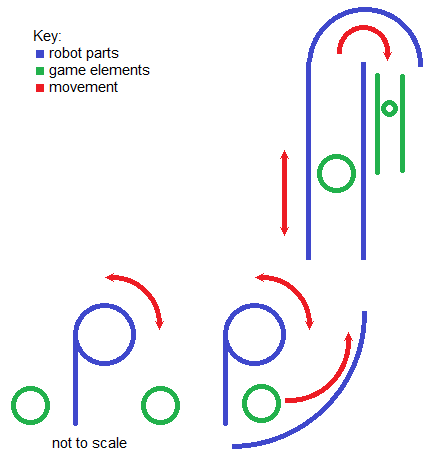
\includegraphics[scale=0.7]{./Entries/Images/scoring_design.png}
\end{center}
